\documentclass[letterpaper, 12pt]{report}
\usepackage[utf8]{inputenc}
\usepackage[spanish]{babel}
\usepackage{cite,url,graphicx,amsmath,amssymb,enumitem,amsthm}
\usepackage{fullpage}
\usepackage{authblk}

%para definir bibliografia en referencias
%\usepackage{etoolbox}
%\makeatletter
%\patchcmd{\thebibliography}{%
%  \chapter*{\bibname}\@mkboth{\MakeUppercase\bibname}{\MakeUppercase\bibname}}{%
%  \chapter*{Bibliografía}}{}{}
%\makeatother

%definición de definicones matemágicas
\newtheorem{defn}{Definición}

%espacio entre párrafos
\setlength{\parskip}{10pt}

%interlineado
%\renewcommand{\baselinestretch}{1.5}

\title{Estudio de algoritmos de calendarización para flujos de trabajo}
\author{Fernando Aguilar Reyes}

\affil{Tesina para obtener el título de Ingeniero en Computación \\
       Instituto Tecnológico Autónomo de México \\
     Río Hondo \#1, Progreso Tizapán, Del. Álvaro Obregón, 01080 \\
     México, Distrito Federal \\}

\begin{document}

\maketitle

\tableofcontents

\listoffigures

\chapter{Introducción}
Cada día, los cómputos son más complejos. Hay bancos que procesan millones de transacciones diarias. Las películas de animación requieren vastos tiempos de cómputo. Muchos proyectos de computación científica requieren hacer numerosos cálculos para llegar a resultados pertinentes. ¿Qué tienen en común todas estas aplicaciones? Ya hemos mencionado que toman mucho tiempo calcularse. Entonces, es natural pensar que se puede distribuir el gran trabajo que requieren estos proyectos entre varias computadoras para disminuir el tiempo total de ejecución y de esta forma, tener una solución escalable. 

Lograr esta paralelización requiere un esfuerzo por parte del desarrollador de la solución. Aunque estas técnicas de paralelización son muy efectivas, éstas son aplicadas cuando el problema a resolver ha sido bien definido y cuando sólo hay una instancia del problema. Ahora bien, cuando la solución involucra varios pasos que están relacionados entre sí, por ejemplo, que el programa C requiera de la salida del programa A y del programa B para que pueda funcionar. O, cuando estamos definiendo los grandes bloques de solución del problema, hay una cierta secuencia que debemos seguir y, dentro de dicha secuencia, hay algunos pasos que podemos resolver de manera concurrente. Por lo tanto, estamos haciendo un \emph{modelo} de nuestro problema.

Este modelo también es llamado \emph{flujo de trabajo}. De manera muy abstracta, un modelo de trabajo es un conjunto de pasos que modelan la ejecución de un proceso. Este concepto ha sido aplicado en numerosas áreas. En el ámbito de los negocios, se utiliza diagramas dibujados con los bloques y reglas del \emph{Bussiness Process Execution Language} para modelar procesos de negocio.

En el ámbito de las ciencias en computación, los flujos de trabajo son aplicados para modelar problemas que requieran varios pasos para su solución. Algunos flujos de trabajo requieren mucho tiempo tiempo de ejecución para sus pasos, como son el caso de los flujos de trabajo científicos. Otros flujos de trabajo son muy simples pero  se requieren que se ejecuten muchos de éstos. De esta forma, es desable distribuir la ejecución de éstos flujos de trabajo entre varias computadoras. Si bien es posible paralelizar algunos pasos de la ejecución de nuestro flujo de trabajo utilizando las técnicas antes mencionadas, hay restricciones de orden que se deben respetar, por lo cual, se debe planear la ejecución del flujo de trabajo.

Hay varias maneras de hacer esta planeación de la ejecución, también llamada \emph{calendarización}. Cabe aclarar que definimos la calendarización como la asignación de recursos a tareas de tal modo que se ejecuten todas las tareas. Con ello, se desea encontrar una forma óptima de hacer esta calendarización, como reducir el tiempo de ejecución total del flujo de trabajo. Sin embargo, con la aparición del cómputo en la nube, es posible ejecutar nuestro flujo de trabajo con otras restricciones, como minimizar el presupuesto necesario para la ejecución del flujo afectando el tiempo de ejecución.

%mencionar instruction level paralelism, task level paralelism, 

%uml, bepl para software y negocios, buscar los que vienen en el paper de hierarchical scheduling for swindew-c

En esta tesina se hace un estudio de los principales algoritmos de calendarización de flujos de trabajo, con énfasis en los algoritimos utilizados en cómputo distribuido, en especial en cómputo en la nube. En el capítulo 2 se habla de un estudio detallado del concepto de flujos de trabajo y su aplicación en computación. El capítulo 3 trata los principales enfoques de cómputo distribuido para ejecutar estos flujos. En el capítulo 4 se hace un estudio de los principales algoritmos de calendarización de los flujos. Finalmente, en el capítulo 6 discutiremos algunas conclusiones sobre el análisis de estos algoritmos.


\chapter{Flujos de trabajo}

\section{Definición y ejemplos}
Un flujo de trabajo es un conjunto de pasos que modelan la ejecución de un proceso \cite{gutierrez2012agent}. En la literatura especializada, los flujos de trabajos también son conocidos como \emph{workflows}. En particular, se estudian a los flujos de trabajo utilizados para vislumbrar la ejecución de un proceso de cómputo. A continuación, se muestran algunos ejemplos de estos flujos de trabajo.

\subsection{Anotación de proteínas}
En el proyecto \emph{e-Protein}, realizado por la Escuela Imperial de Londres, se realizó un flujo de trabajo para la anotación de proteínas. El objetivo del proyecto \cite{o2004mapping} era la identificación y anotación de partes de proteínas que expliquen su estructura y su función. En la figura \ref{fig:iceni-workflow} se muestra el flujo de trabajo desarrollado, donde las cajas representan los programas que son ejecutados para cada paso del proceso de anotación, y las líneas que conectan a las cajas representan las dependencias de datos entre los programas, es decir, si una caja tiene una línea que apunta a ella, significa que dicho programa depende de otro porgrama determinado por el otro extremo de la flecha.

\begin{figure}
    \begin{center}
        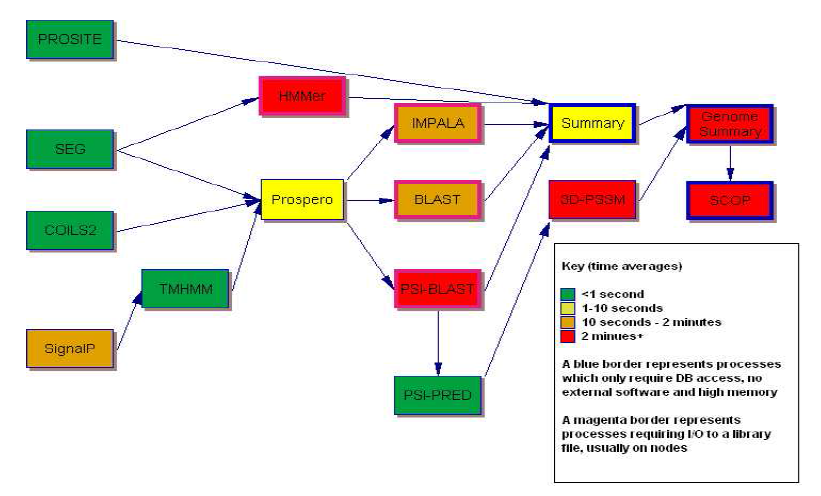
\includegraphics[width=0.8\textwidth]{imagenes/iceni-workflow}
    \end{center}
    \caption{Flujo de trabajo para la anotación de proteínas, diseñado en la Escuela Imperial de Londres para el proyecto \emph{e-Protein}.}
    \label{fig:iceni-workflow}
\end{figure}


\subsection{Curvas de amenaza sísmica}
Otro notable ejemplo es el proceso para generar curvas de amenaza que describen las probabilidades de que ocurra un temblor en una determinada área. Para elaborar estas curvas, los científicos del Centro de Terremotos del Sureste de California (SCEC por sus siglas en inglés) tienen que realizar una gran cantidad de simulaciones para que sus resultados puedan ser combinados y expresados en la curva de amenaza \cite{deelman2006managing}. El flujo de trabajo para generar la curva de amenaza se muestra en la figura \ref{fig:scec-workflow}.

\begin{figure}
    \begin{center}
        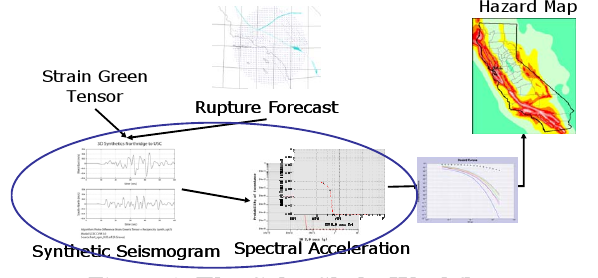
\includegraphics[width=0.8\textwidth]{imagenes/scec-workflow}
    \end{center}
    \caption{Flujo de trabajo para generar curvas de amenaza, elaborado por el SCEC.}
    \label{fig:scec-workflow}
\end{figure}

\subsection{Generación de facturas}
Recientemente en México, el Sistema de Administración Tributaria emitió los lineamientos para que las operaciones de compra-venta entre personas físicas y morales puedan ser registradas por medio de facturas electrónicas. Para generar estos Comprobantes Fiscales Digitales, las empresas tienen que hacer procesos de validaciones de RFC y encriptar el contenido de la factura con un mecanismo de llave privada. Naturalmente, este proceso de generación de factura requiere de varias actividades. En la figura \ref{fig:cfd-workflow} se muestra el flujo de trabajo que utiliza una empresa para generar sus facturas. Este flujo se encuentra documentado en una tesina presentada por Alcerreca \cite{alcerreca2013cfd}.

\begin{figure}
    \begin{center}
        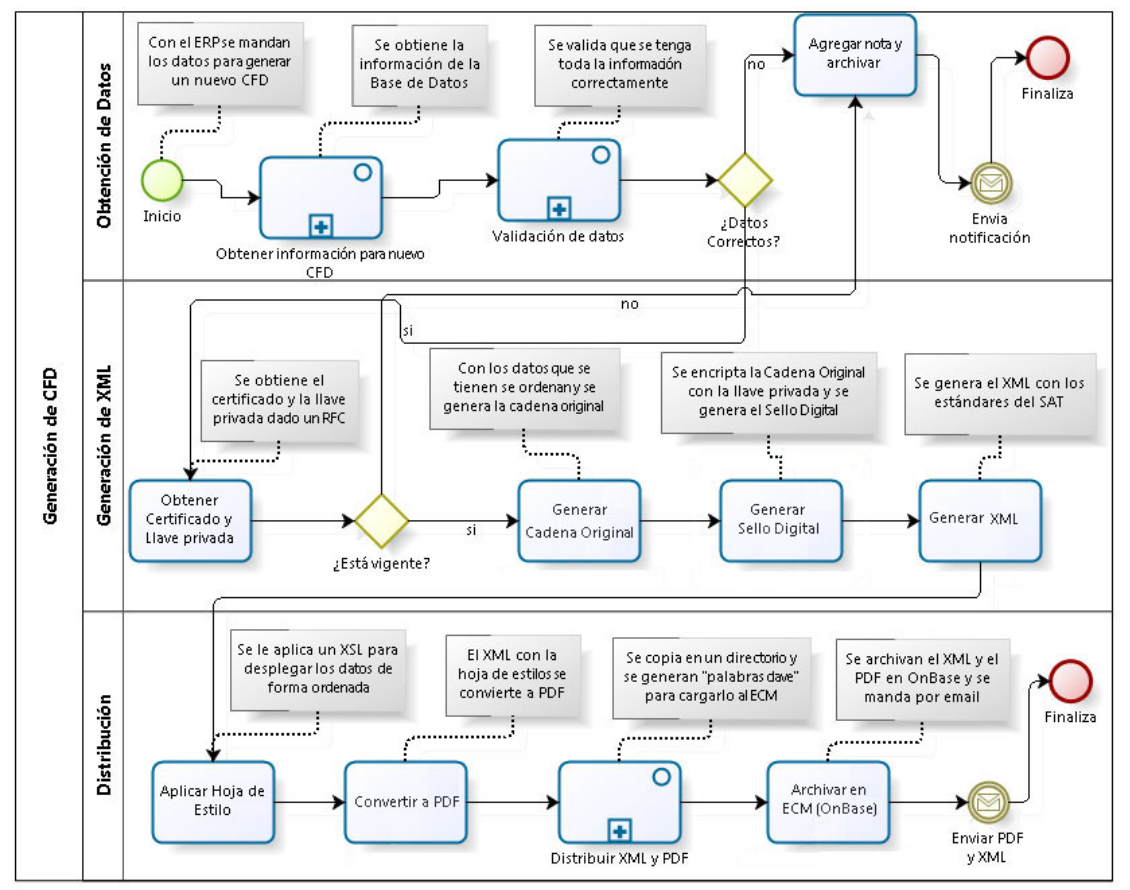
\includegraphics[width=0.8\textwidth]{imagenes/cfd-workflow}
    \end{center}
    \caption{Flujo de trabajo para generar facturas electrónicas, utilizado por una empresa de cementos.}
    \label{fig:cfd-workflow}
\end{figure}


\section{Estructura de los flujos de trabajo}
Como hemos visto en los dos ejemplos anteriores, los flujos de trabajo presentados describen los \emph{pasos} que necesitan para calcular la solución de un problema. En éstos, no se ha hablado sobre detalles para hacer los cómputos necesarios para cada flujo. Tampoco definen las plataformas de cómputo en que se ejecutan estos flujos. Tan sólo definen los grandes pasos para solucionar el problema y las dependencias que tienen estos pasos. 

Ahora, es muy común que estas dependencias estén dictadas por los datos que requiere cada paso para funcionar. Sin embargo, hay situaciones en los que los pasos del flujo no requieren los datos del paso anterior para funcionar, sino que las dependencias están marcadas por el orden temporal que deben seguir estos pasos. Así, se puede notar una ambigüedad en la definición de un flujo de trabajo.

\subsection{Perspectivas de los flujos de trabajo}
El trabajo de Van der Aalst et al. \cite{van2003workflow} identifica una serie de perspectivas vislumbrados en las definiciones de las especificaciones de un flujo de trabajo en las que se basan los sistemas que administran la ejecución de éstos. Las cuatro perspectivas se enuncian a continuación:
%En esta tesis, tomaremos estas perspectivas a manera de una clasificación de flujos de trabajo basadas en la forma en que describen sus dependencias

\begin{itemize}

\item{\textbf{Perspectiva de control de flujo.} Describe las relaciones de las actividades (pasos) con estructuras de control, tales como: secuencia, decisión, ejecución de actividades en paralelo y punto de sincronización conjunta\footnote{Esta estructura de control también es conocida como \emph{join synchronization}}.}

\item{\textbf{Perspectiva de datos.} En ella, los flujos de trabajo describen las entradas y salidas de datos, tanto de ejecución como de control, que se tienen en cada actividad del flujo. También se toma en cuenta los datos locales a cada actividad; es decir, que sólo son necesarios dentro del contexto de ésta.}

\item{\textbf{Perspectiva de recursos.} Muestra cuáles son los recursos con los que se cuentan para ejecutar el flujo de trabajo y la forma en que estos recursos se encuentran organizados. Estos recursos pueden ser desde entidades de cómputo hasta roles con responsabilidades específicas cumplidas por actores humanos.}

\item{\textbf{Perspectiva operacional.} Aquí se detallan las operaciones elementales necesarias en cada actividad para ejecutar el flujo de trabajo. Estos detalles incluyen las transferencias de datos entre las operaciones y su correspondencia en programas.}

\end{itemize}

Cabe aclarar que estas perspectivas están relacionadas entre sí de modo que el control de flujo es la base en la que descansan las demás perspectivas. Esto es porque la perspectiva de datos requiere que el control de flujo tenga los datos de entrada y salida como prueba de que se cumplieron las pre y post-condiciones de cada actividad, respectivamente; la perspectiva de recursos define con qué se ejecutarán y almacenará los datos del flujo de trabajo; mientras que la perspectiva operacional trata los detalles sobre cómo se utilizan \emph{físicamente} los recursos, los datos y los programas a lo largo del flujo de trabajo.

\section{Calendarización como control de flujo}

El hecho de que la perspectiva de control de flujo sea la base de las demás perspectivas indica que la forma en que controla la ejecución del flujo determina de manera fundamental el rendimiento de la ejecución total de una instancia del flujo. Por lo tanto, es de vital importancia encontrar métodos de calendarización que permitan encontrar correspondencias entre recursos y actividades que cumplan con los requisitos dictados en las especificaciones examinadas en la perspectiva del control del flujo y que también maximicen el rendimiento de la ejecución de todo el flujo en general.

En este trabajo, se establecerán las siguientes consideraciones para limitar el estudio de los algoritmos de calendarización, a saber:

\begin{itemize}
\item{Los flujos de trabajo están representados como \emph{grafos dirigidos acíclicos}, con el objetivo de simplificar el estudio}

\item{Las tareas (o actividades) de los flujos de trabajo son consideradas \emph{atómicas}, i.e., una tarea no puede ejecutarse incompletamente. Algunos sistemas de administración de ejecución de flujos de trabajo tienen mecanismos para lidiar con estos errores, pero el estudio de éstos queda fuera de los límites de este trabajo.}

\item{La información de las \emph{demás perspectivas} se puede requerida, dependiendo si el mecanismo de calendarización lo considere necesario para tomar mejores decisiones.}
\end{itemize}

%conclusiones:
% - representar como DAG's porque es sencillo y expresivo (balanceado)
% - tareas atómicas
% - la información de las demás perspectivas se puede requerir o no, dependiendo de como lo requiera el calendarizador.


%ejemplo: ICENI tiene partes paralelas, que no requieren de ciertos datos para operar
%ejemplo: Si hablas de orden,
%poner ejemplos donse se ejemplifique esta calendarización

%clasificados de acuerdo a dependencias (de orden, o de datos)


%clasificados de acuerdo a nivel de detalle (específico para cada plataforma)

%clasificados de acuerdo a instancias
% - pocas instancias, mucho tiempo de cómputo:
% - intensivos en instancias, pero cortos en ejecución:

%todos se pueden representar como Grafos Dirigidos Acíclicos

%implementaciones de representación de workflows
% - AGWL


\chapter{Cómputo distribuido}
Los flujos de trabajo requieren de recursos de cómputo para su ejecución. En los ejemplos anteriores se mencionaron aplicaciones científicas que, por su naturaleza, requieren vasto tiempo de ejecución para llevarse a cabo. Por otro lado, también existen aplicaciones de negocio que, si bien son computacionalmente sencillas, se requiere ejecutar una gran cantidad de instancias de estos flujos de trabajo. Por ello, ejecutar cualquiera de estos flujos de trabajo en una sola computadora resulta prohibitivo. Así, se hace uso de varias computadoras para distribuir el esfuerzo para correr estos grandes procesos.

Dependiendo de cómo estén organizados estas computadoras, se definen los enfoques para correr los flujos de trabajo con cómputo distribuido.

\section{Enfoques de cómputo para flujos de trabajo}
Diversos enfoques se han aplicado para distribuir la ejecución de un flujo de trabajo entre varias computadoras.  De acuerdo a Buyya et al., los enfoques de cómputo más importantes para los flujos de trabajo son los \emph{clusters}, los \emph{grids} y las \emph{nubes} \cite{buyya2009cloud}. A continuación, explicaremos cada uno de los enfoques.

\subsection{Clusters}
Los \emph{clusters} son sistemas distribuidos, paralelos, compuestos de varias computadoras que son vistas como un único recurso de cómputo \cite{buyya2009cloud}. 

Un ejemplo de un cluster es la instalación de la Universidad Autónoma Metropolitana, campus Iztapalapa, llamada \emph{Aitzaloa}, compuesta por 270 nodos de cómputo, cada uno equipado con dos procesadores Intel Xeon Quad-Core y 16GB en RAM; los nodos están conectados entre sí por medio de switches Ethernet e Infiniband. El cluster también cuenta con un sistema de archivos distribuido basado en Lustre. La capacidad real de cómputo del cluster Aitzaloa es de 18.4 teraFLOPS \cite{uamz2013tizaloa}.

El detalle de la topología del cluster se puede apreciar en la figura \ref{fig:topologia_aitzaloa}, en donde podemos apreciar que los switches son los puntos de conexión entre el nodo maestro, el sistema de almacenamiento distribuido y los nodos de cómputo.

\begin{figure}
    \begin{center}
        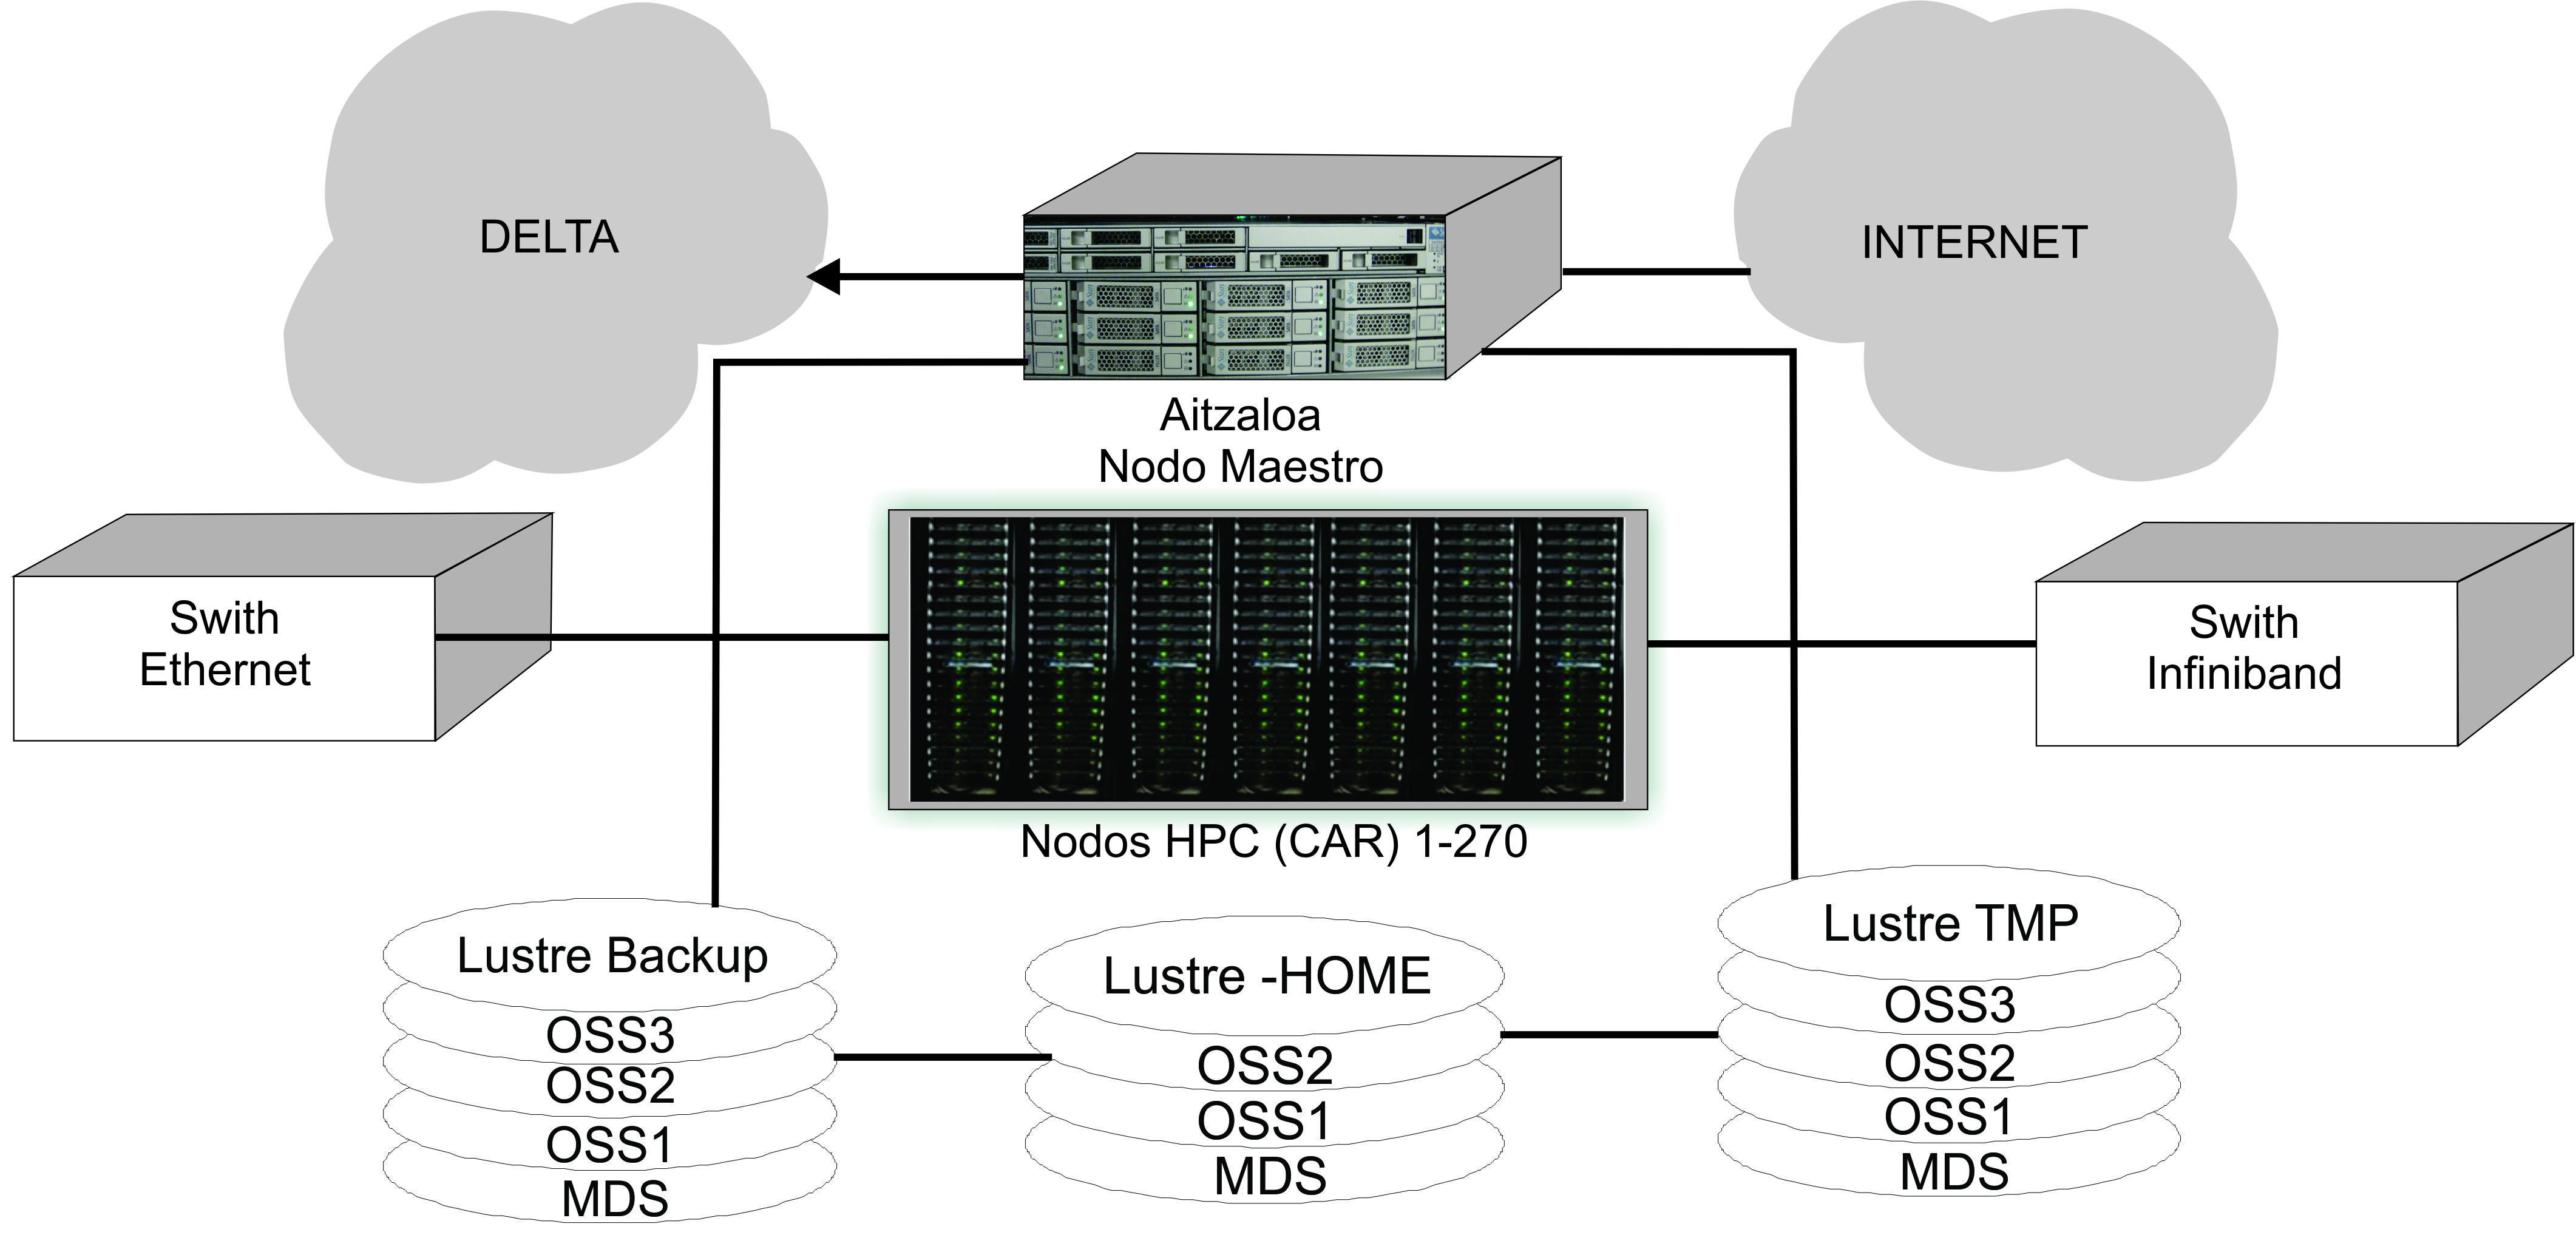
\includegraphics[width=0.8\textwidth]{imagenes/topologia_aitzaloa}
    \end{center}
    \caption{Topología del cluster Aitzaloa}
    \label{fig:topologia_aitzaloa}
\end{figure}


\subsection{Grids}
Los \emph{grids} son sistemas distribuidos, paralelos, compuestos de computadoras autónomas y geográficamente distribuidas que pueden trabajar en conjunto o de manera independiente de acuerdo a los objetivos, políticas y mecanismos de uno o varios administradores del sistema, es decir, un grid puede ser compartido entre varias instituciones \cite{buyya2009cloud}. 

El proyecto \emph{LANCAD}\footnote{Laboratorio Nacional de Cómputo de Alto Rendimiento} es un buen ejemplo, pues une el cluster \emph{Aitzaloa} de la UAM, el cluster de la UNAM \emph{KamBalam}, y el cluster \emph{Xiuhcoatl} del CINVESTAV por medio de una red de fibra óptica instalada en las estaciones del Sistema de Transporte Colectivo Metro. La suma de la potencias reales de cada \emph{nodo robusto} del grid es de 48.55 teraFLOPS \cite{lancad2013xiuhcoatl}.

En la figura \ref{fig:LANCAD-mapa-fo} se muestra los tramos de línea de Metro que cuentan con fibra óptica para conectar cada uno de las supercomputadoras (clusters) de las tres instituciones.

\begin{figure}
    \begin{center}
        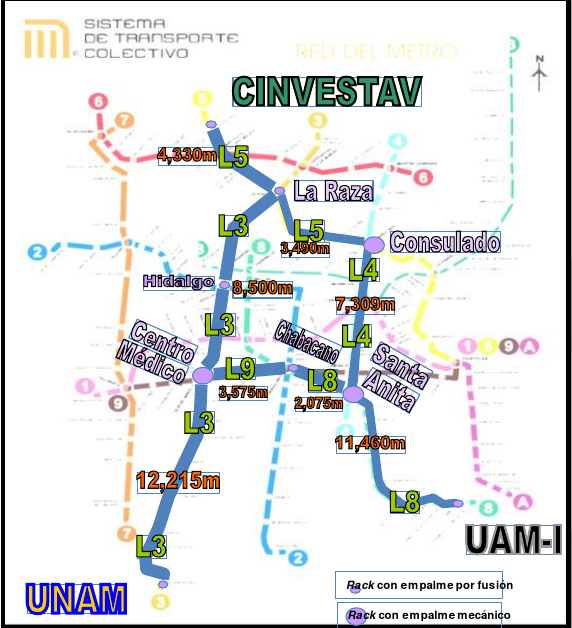
\includegraphics[width=0.8\textwidth]{imagenes/LANCAD-mapa-fo}
    \end{center}
    \caption{Detalle de la red de fibra óptica para conectar los nodos robustos del grid del proyecto LANCAD}
    \label{fig:LANCAD-mapa-fo}
\end{figure}


\subsection{Nubes}
Las \emph{nubes} (clouds) son sistemas distribuidos, paralelos, compuestos de computadoras o máquinas virtuales interconectadas que son aprovisionadas para usarse como uno o varios recursos de cómputo, de acuerdo a un contrato de nivel de servicio acordado entre el proveedor de la nube y el cliente \cite{buyya2009cloud}. 

Empresas nuevas y existentes proveen servicios de cómputo en la nube, tales como GoGrid, Rackspace, Amazon, Microsoft, IBM, Oracle, entre otras. La forma en que operan es la siguiente: se paga cierta cantidad por utilizar servicios de cómputo o almacenamiento durante determinado tiempo. Así, los clientes no tienen que invertir grandes cantidades de dinero para contar con una gran infraestructura como en el caso de los los clusters y los grids.

\section{Comparación de los enfoques}
Si bien estos enfoques difieren, principalmente, en la forma en que están organizadas las unidades de cómputo, podemos enumerar algunas observaciones.

Primero, es natural ver que los grids están compuestos de clusters, pero también podría verse a un grid como un gran cluster. Hasta cierto punto este razonamiento parece correcto. Sin embargo, la diferencia importante entre clusters y grids radica en el hecho de que el grid es comúnmente administrado por varios técnicos de varias instituciones que, pueden tener objetivos y necesidades diversas, mientras que un cluster requiere de menos administradores y se asume una mayor flexibilidad para enfrentar los fallos de un cluster.

Segundo, tanto los grids como las nubes son físicamente muy similares: ambos consisten de varios clusteres interconectados y distribuidos geográficamente. Entonces, ¿cuál es la diferencia? Lo que distingue a las nubes de los grids son dos características: (1) en una nube, se utilizan \emph{máquinas virtuales} para distribuir el recurso. El usuario tiene la vista de una parte del grid como si fuera una computadora dedicada exclusivamente para éste. Por otro lado, en los grids, es común que el usuario acceda a él con una cuenta asignada por un administrador, de tal suerte que se tiene una vista de una gran máquina que es compartida entre varios usuarios. Muchos de los administradores de grids en el mundo administran los trabajos encargados por los usuario de tal modo que se ejecuten lo más rápido posible con los recursos disponibles en un tiempo dado. Los usuarios, en algunos casos obtienen acceso al grid y trabajan sus proyectos de manera gratuita o, en caso contrario, pagan una cuota por un tiempo fijo de cómputo. Pero, en el caso de las nubes, se agrega un modelo económico para acceder a los recursos llamado \emph{pay as you go}, en donde el usuario paga una cuota por los recursos utilizados, sin alguna limitación mas que el presupuesto. Asi, el usuario podría pagar una gran cantidad para que su flujo de trabajo se ejecute en el menor tiempo posible o también podría pagar una menor cantidad sacrificando el tiempo total de ejecución del flujo.


\chapter{Calendarización}
La calendarización\footnote{También conocida en la literatura especializada como \emph{scheduling}} es el proceso de asignación de recursos a tareas, de tal modo que se define un orden de ejecución de las tareas, teniendo lugar diferentes combinaciones de recursos y tareas. En este capítulo se define de la forma más elemental el problema de la calendarización para estudiar sus propiedades y también se explica la relación de este problema fundamental con los flujos de trabajo.

\section{Definición del problema}
De acuerdo a  Ullman et al. \cite{ullman1975np}, el problema de la calendarización se define de la siguiente manera: 

%al parecer hay que usar la definición extendida de Ullman para que muestre a la calendarización como una función f
\begin{defn}
El \textbf{problema de la calendarización} consiste en:
\begin{enumerate}
\item Un conjunto de tareas $S = \{ J_1, J_2, \dots, J_n \}$
\item Un ordenamiento parcial $\prec$ sobre $S$
\item Una función de costo $W: S \mapsto \mathbb{Z}^{+}$, la cual indica el tiempo que tarda en completarse cada una de las tareas en $S$
\item Un número de computadoras (procesadores) $k$
\end{enumerate}
Para este caso, se asume que cuando una computadora ejecuta una tarea, ésta es ejecutada completamente. Así, el objetivo es \emph{minimizar} el tiempo total de ejecución, denotado por $t_\text{max}$, respetando el orden parcial definido por $\prec$.
\end{defn}


\section{La complejidad de calendarizar}
Como puede notarse, hay varias maneras de acomodar las $k$ computadoras para que se ejecuten todas las tareas de $S$. Sin embargo, Ullman et al. han demostrado que este problema pertenece a la categoría NP-completo \cite{ullman1975np}.

Esto signifca que no se ha encontrado un algoritmo que pueda resolver el problema en tiempo polinomial. Entonces, la solución ingenua de probar ordenadamente todas las posibles asignaciones de tareas a computadoras resulta computacionalmente muy caro.

Así, la forma de atacar estos problemas NP-completos es utilizar métodos de aproximación \cite{leiserson2001introduction} que obtengan soluciones subóptimas o utilizar heurísticas que resuelvan este problema sumando ciertas restricciones.

\section{Calendarización de flujos de trabajo}
Hasta ahora, se ha mencionado el problema básico de calendarización con restricciones. Con ello, se pretende plantear el problema de la calendarización de flujos de trabajo y apoyarse en la definición del problema básico de calendarización para enumerar propiedades sobre este problema.

Para plantear el problema de la calendarización de flujos de trabajo, primero se demostrará que bajo ciertas condiciones, un flujo de trabajo puede ser reducido a un grafo dirigido acíclico haciendo las transformaciones adecuadas. Luego, se utilizará la definición del problema básico de calendarización con restricciones y su semejanza para flujos de trabajo. Finalmente, se hará una descripción de la complejidad de calendarizar flujos de trabajo.
%tres hechos:
% - todo flujo de trabajo puede reducirse a DAG
% - transforma un DAG a un problema clásico de Ullman
% - menciona que el problema de Ullman es NP-completo
\subsection{Reducción de flujos de trabajo a grafos dirigidos acíclicos}
En el trabajo de de Mair et al. \cite{mair2007workflow} proponen un formato para una representación intermedia de flujos de trabajo, con el fin de transformar una especificación de un flujo de trabajo detallada --escrita en un lenguaje basado en XML llamado AGWL-- a una representación intermedia basada en grafos dirigidos acíclicos.

Aunque no existe un consenso general sobre cuál es una definición completa de un flujo de trabajo \cite{van2003workflow}, el lenguaje AGWL es una especificación suficiente para una gran cantidad de flujos de trabajo de ámbito científico, porque con las construcciones if, while, for, parallel, secuence son adecuadas para expresar vastos flujos.

El hecho importante a recalcar es que los grafos dirigidos acíclicos sirven como representación para utilizarlos en los algoritmos de calendarización.


\subsection{Definición del problema de calendarización de flujos de trabajo}
Una vez que se ha establecido a los grafos dirigidos acíclicos como nuestra representación básica de flujos de trabajo, se definirá el problema que conlleva asignar recursos a las tareas del flujo.

Con el fin de no perder generalidad, tomaremos la definición de Wieczorek-Prodan \cite{wieczorek2008taxonomies} del problema:

\begin{defn}
Un \textbf{flujo de trabajo} es un grafo dirigido $w \in \mathcal{W}, w = (\mathcal{V},\mathcal{E})$, compuesto de un conjunto de nodos $\mathcal{V}$ y un conjunto de aristas $\mathcal{E}$, donde los nodos y las aristas representan tareas $ \tau \in \mathcal{T}$ y transferencias de datos $ \rho \in \mathcal{D}$.
\end{defn}

Hay que notar que en la definición anterior que la forma en que se relacionan las tareas y las transferencias de datos con los nodos y aristas del grafo está determinada por la representación \emph{concreta} del flujo de trabajo.
%creo que esto requiere más trabajo.

Ahora, se definirán los recursos de cómputo en donde se ejecuta el flujo. La definición de Wieczorek-Prodan habla de grids, pero es fácilmente aplicable a otros enfoques de cómputo

\begin{defn}
Un \textbf{servicio} es una entidad de cómputo que puede ejecutar una tarea $\tau \in \mathcal{T}$. El conjunto de todos los servicios disponibles para ejecutar el flujo de trabajo está denotado por $\mathcal{S}$.
\end{defn}

De este modo, la calendarización es definida como una función:

\begin{defn}
La \textbf{calendarización de un flujo de trabajo} $w$ es una función $ f: \mathcal{T} \mapsto \mathcal{S}$ que asigna servicios a las tareas del flujo. El conjunto que contiene todas las posibles calendarizaciones de $w$ es denotado por $\mathcal{F}$.
\end{defn}

Cada posible calendarización determina un costo de ejecución. A continuación, definiremos el modelo de costo determinado por la utlización de los servicios.

\begin{defn}
Un \textbf{modelo de costos} es un conjunto de criterios $C = \{c_1, c_2, \dots, c_n\}$ que determinan las restricciones en las que se debe ejecutar una calendarización, por ejemplo, un límite en el tiempo de ejecución, en el costo monetario o la tolerancia a fallos, entre otros.
\end{defn}

\begin{defn}
Para cada criterio $c_i \in C$, existe una \textbf{función de costo parcial} $\Theta_i : \mathcal{S} \mapsto \mathbb{R}$, en la que a cada servicio disponible para ejecutar el flujo de trabajo se le asocia un costo por ejecutar dicho servicio con las restricciones dictadas con el criterio $c_i$.
\end{defn}

\begin{defn}
Para cada criterio $c_i \in C$, existe una \textbf{función de costo total} $\Delta_i : \mathcal{W} \times \mathcal{F} \mapsto \mathbb{R}$, que asigna un flujo de trabajo $w$ calendarizado por $f$ un costo basado en los costos parciales determinados por los servicios utlizados para ejecutar las tareas del flujo.
\end{defn}

El objetivo del problema de la calendarización de flujos de trabajo es encontrar la calendarización $f$ que minimice las funciones de costo total $\Delta_i$, $1 \le i \le n$.

\subsection{Complejidad computacional de la calendarización de flujos de trabajo}
Después de haber enunciado varias definiciones para definir el problema de la calendarización de flujos de trabajo, se hará una analogía con el problema básico de calendarización para poder estudiar su complejidad computacional. La analogía es la siguiente:


\begin{enumerate}
\item El conjunto de tareas $S$ equivale a las tareas $\mathcal{T}$ descritas por el flujo de trabajo.

\item El ordenamiento parcial $\prec$ está representado tanto por las dependencias de datos $\mathcal{D}$ y las aristas $\mathcal{E}$ que representan el control de flujo que debe respetarse para ejecutar el flujo.

\item Las $k$ computadoras equvivalen al conjunto de servicios $\mathcal{S}$ disponibles para ejecutar el flujo.

\item La función de costo $W$ tiene una equivalencia implícita. El problema básico asume que conocemos apriori el tiempo de ejecución de una tarea. Sin embargo, es muy frecuente que sólo tengamos una estimación del tiempo de ejecución. Por otro lado, podemos establecer una función auxiliar que relacione las tareas con los servicios. Dicha relación es la función de calendarización $f$. En efecto, ejecutar una tarea en un servicio genera un costo, determinado por las funciones parciales y totales. Por lo pronto, estableceremos una relación proporcional entre costo y tiempo, con el fin de mostrar que existe una equivalencia entre la función de costo $W$ del problema básico y el modelo de costo de un flujo de trabajo.
\end{enumerate}

Con lo anterior, hemos establecido que el problema de la calendarización de flujos de trabajo es equivalente al problema básico de calendarización. Entonces, es natural inferir que el problema de la calendarización de flujos de trabajo pertenece a la categoría de problemas NP-completo.

%tareas -> servicios -> costo <=> tiempo

\chapter{Algoritmos de calendarización de flujos de trabajo}
En el capítulo anterior definimos el problema de calendarizar flujos de trabajo. También se vio que dicho problema pertenece a la categoría de los problemas NP-completo, lo cual significa que la complejidad --o tiempo de ejecución-- para resolver este problema no está acotada por una función polinomial. Por ello, diversos algoritmos se han propuesto para atacar, ya sea de manera total o parcial, el objetivo principal de la calendarización: optimizar el tiempo de ejecución total.

Ahora, con los enfoques de cómputo propuestos en el capítulo 2, se crean diversos algoritmos para diferentes necesidades. Mientras que en los clusters y los grids se asumen que estos recursos son compartidos, los algoritmos de calendarización para estos recursos asumen que los flujos deben ser ejecutados lo más pronto posible, con el fin de hacer que el recurso esté ocupado la mayor parte del tiempo. Por otro lado, el enfoque de nubes permite diseñador de flujos de trabajo elegir entre ejecutar el flujo con todos los recursos a costa de un elevado presupuesto o, minimizar dicho presupuesto tolerando un tiempo de ejecución mayor al mínimo posible.

De acuerdo a Yu et al. \cite{yu2008workflow}, se pueden clasificar los algoritmos de calendarizar los algoritmos de flujos de trabajo ejecutados en grids en dos grandes niveles: los algoritmos de mejor esfuerzo son aquellos que tratan de minimizar el tiempo total de ejecución\footnote{También conocido como \emph{makespan}}, haciendo uso de todos los recursos disponibles. El segundo grupo son los algoritmos de Calidad en el Servicio\footnote{En la literatura especializada se conoce a este término como \emph{Quality of Service}}, los cuales tratan de obtener una calendarización que cumpla las restricciones especificadas como una medida de calidad, con la posibilidad de elegir soluciones que tomen un tiempo de ejecución subóptimo.

A continuación, mostraremos los algoritmos descritos en el trabajo de Yu et al., con los ajustes en notación necesarios para que coincidan con las definiciones de flujo de trabajo establecidas en los capítulos anteriores.


\section{Algoritmos de Mejor Esfuerzo}


\subsection{Myopic (miope)}

\subsection{Min-min}
\subsection{Max-min}
\subsection{Algoritmos genéticos}

\section{Algoritmos de Calidad en el Servicio}
\subsection{Heurítsicas}
\subsection{Metaheurísticas}

\chapter{Software para la administración y ejecución de flujos de trabajo}

\section{Software orientado a clusters}

\subsection{Open Grid Scheduler}

\section{Software orientado a grids}

\subsection{SwinDew-G}

\subsection{Pegasus}

\section{Software orientado a nubes}

\subsection{ANEKA}

\subsection{SwinDew-C}

\subsection{ASKALON}


\chapter{Conclusiones}

%%\renewcommand*{\bibname}{\chapter*{Referencias}}
\bibliographystyle{plain}
\bibliography{propuesta}

\end{document}